\section{Results}

\subsection{Stage 1: loss, sampling, and augmentation screen}

Table~\ref{tab:stage1} reports the Stage 1 screen on EfficientNet-B0 at 160 pixels. The validation winner is CE with strong augmentation, with a validation sensitivity of $0.556\pm0.027$ at 95\% specificity. The CE baseline reaches $0.536\pm0.016$. The planned focal loss with class-balanced sampling reaches $0.502\pm0.039$, and focal loss with $\gamma=3$ and class-balanced sampling reaches $0.449\pm0.051$.

The planned imbalance correction did not beat the CE baseline on validation. The difference between the CE baseline and the strong-augmentation variant is small relative to the seed standard deviation. The test columns in Table~\ref{tab:stage1} are descriptive; the model selection used validation only.

\begin{table}[t]
\centering
\small
\caption{Stage 1 screen on EfficientNet-B0 at 160 pixels. Validation sensitivity is used for model selection. Validation values are mean and standard deviation across three seeds. Test sensitivity is the mean with a 95\% t interval across three seeds at the validation-selected 95\% specificity threshold.}
\label{tab:stage1}
\resizebox{\textwidth}{!}{%
\begin{tabular}{lccccc}
\toprule
Configuration & Val sens & Test sens (95\% t CI) & Specificity & Balanced acc & AUC \\
\midrule
stage1\_ce\_random\_strong & 0.556 $\pm$ 0.027 & 0.513 (0.492 to 0.533) & 0.943 & 0.728 & 0.901 \\
stage1\_ce\_random & 0.536 $\pm$ 0.016 & 0.530 (0.470 to 0.591) & 0.948 & 0.739 & 0.897 \\
stage1\_ce\_cb & 0.521 $\pm$ 0.086 & 0.484 (0.403 to 0.565) & 0.938 & 0.711 & 0.890 \\
stage1\_focal2\_random & 0.509 $\pm$ 0.041 & 0.487 (0.433 to 0.541) & 0.946 & 0.717 & 0.894 \\
stage1\_focal2\_cb & 0.502 $\pm$ 0.039 & 0.480 (0.361 to 0.600) & 0.943 & 0.712 & 0.897 \\
stage1\_wce\_random & 0.502 $\pm$ 0.043 & 0.493 (0.430 to 0.556) & 0.937 & 0.715 & 0.896 \\
stage1\_focal2\_cb\_strong & 0.483 $\pm$ 0.013 & 0.491 (0.274 to 0.708) & 0.943 & 0.717 & 0.896 \\
stage1\_focal3\_cb & 0.449 $\pm$ 0.051 & 0.478 (0.430 to 0.527) & 0.946 & 0.712 & 0.899 \\
\bottomrule
\end{tabular}
}
\end{table}


\subsection{Stage 2: architecture comparison}

Table~\ref{tab:stage2} reports the Stage 2 comparison at 224 pixels. The three conditions are the CE baseline, focal loss with class-balanced sampling, and CE with strong augmentation.

At the CE baseline, ResNet-50 reaches a test sensitivity of $0.570$ (95\% t interval $0.469$ to $0.671$), EfficientNet-B0 reaches $0.556$ ($0.465$ to $0.646$), and ViT-S/16 reaches $0.400$ ($0.291$ to $0.508$). The two CNNs lead the transformer in the point estimates, but the intervals overlap.

Under focal loss with class-balanced sampling, ResNet-50 falls to $0.453$ ($0.289$ to $0.618$), EfficientNet-B0 falls to $0.477$ ($0.295$ to $0.658$), and ViT-S/16 rises to $0.482$ ($0.428$ to $0.536$). The correction changes the point estimates by $+8.2$ points for the transformer and by $-11.7$ and $-7.9$ points for the two CNNs.

Strong augmentation is close to neutral. ResNet-50 reaches $0.568$ ($0.495$ to $0.642$), EfficientNet-B0 reaches $0.563$ ($0.402$ to $0.724$), and ViT-S/16 reaches $0.435$ ($0.228$ to $0.643$).

Table~\ref{tab:ranking} reports the seed-level paired comparisons. Every ResNet-50 and EfficientNet-B0 seed falls under focal loss, and every ViT-S/16 seed rises, but all three within-architecture 95\% t intervals include zero. The difference-in-differences is $-0.161$ ($-0.209$ to $-0.113$) for EfficientNet-B0 minus ViT-S/16 and $-0.199$ ($-0.484$ to $0.087$) for ResNet-50 minus ViT-S/16. The EfficientNet-B0 versus ViT interaction is therefore significant at the seed level; the ResNet-50 versus ViT interaction is directionally consistent but not significant.

The point-estimate ranking reverses, but the evidence supports an architecture-dependent interaction with limited precision, not a definitive ordering. The same caveat applies to the strong-augmentation changes, whose intervals all include zero.

At a common 95\% test specificity, the CE CNNs reach $0.581$ and $0.575$ against $0.348$ for the ViT. Under focal loss the values are $0.450$, $0.466$, and $0.437$. The ViT gain and the CNN loss therefore persist at a matched operating point, not only at the validation-selected threshold.

\begin{table}[t]
\centering
\small
\caption{Stage 2 comparison at 224 pixels. Validation values are mean and standard deviation across three seeds. Test sensitivity is the mean with a 95\% t interval across three seeds at the validation-selected 95\% specificity threshold.}
\label{tab:stage2}
\resizebox{\textwidth}{!}{%
\begin{tabular}{lccccc}
\toprule
Configuration & Val sens & Test sens (95\% t CI) & Specificity & Balanced acc & AUC \\
\midrule
stage2\_efficientnet\_b0\_ce\_random\_strong & 0.521 $\pm$ 0.021 & 0.563 (0.402 to 0.724) & 0.952 & 0.757 & 0.912 \\
stage2\_efficientnet\_b0\_ce\_random & 0.553 $\pm$ 0.035 & 0.556 (0.465 to 0.646) & 0.953 & 0.754 & 0.914 \\
stage2\_efficientnet\_b0\_focal2\_cb & 0.481 $\pm$ 0.042 & 0.477 (0.295 to 0.658) & 0.950 & 0.713 & 0.891 \\
stage2\_resnet50\_ce\_random & 0.526 $\pm$ 0.044 & 0.570 (0.469 to 0.671) & 0.951 & 0.761 & 0.897 \\
stage2\_resnet50\_ce\_random\_strong & 0.549 $\pm$ 0.015 & 0.568 (0.495 to 0.642) & 0.942 & 0.755 & 0.899 \\
stage2\_resnet50\_focal2\_cb & 0.489 $\pm$ 0.027 & 0.453 (0.289 to 0.618) & 0.947 & 0.700 & 0.884 \\
stage2\_vit\_s\_focal2\_cb & 0.474 $\pm$ 0.034 & 0.482 (0.428 to 0.536) & 0.940 & 0.711 & 0.872 \\
stage2\_vit\_s\_ce\_random\_strong & 0.466 $\pm$ 0.030 & 0.435 (0.228 to 0.643) & 0.941 & 0.688 & 0.866 \\
stage2\_vit\_s\_ce\_random & 0.423 $\pm$ 0.042 & 0.400 (0.291 to 0.508) & 0.941 & 0.670 & 0.854 \\
\bottomrule
\end{tabular}
}
\end{table}

\begin{table}[t]
\centering
\small
\caption{Seed-level paired sensitivity comparisons. Intervals are 95\% t intervals across three seeds. The direction column counts the seeds with the stated sign. The EfficientNet-B0 versus ViT interaction is the only mean difference whose interval excludes zero; the other intervals include zero, so the study is underpowered for a precise ranking.}
\label{tab:ranking}
\resizebox{\textwidth}{!}{%
\begin{tabular}{llccc}
\toprule
Test & Architecture & $\Delta$ sensitivity & 95\% t CI & Direction \\
\midrule
Focal+CB vs CE & EfficientNet-B0 & -0.079 & -0.219 to +0.061 & 3/3 negative \\
Focal+CB vs CE & ResNet-50 & -0.116 & -0.272 to +0.039 & 3/3 negative \\
Focal+CB vs CE & ViT-S/16 & +0.082 & -0.079 to +0.244 & 3/3 positive \\
CE+strong vs CE & EfficientNet-B0 & +0.007 & -0.244 to +0.258 & 2/3 positive \\
CE+strong vs CE & ResNet-50 & -0.002 & -0.069 to +0.065 & 2/3 negative \\
CE+strong vs CE & ViT-S/16 & +0.036 & -0.075 to +0.147 & 2/3 positive \\
\midrule
Difference in differences & EfficientNet-B0 minus ViT-S/16 & -0.161 & -0.209 to -0.113 & 3/3 negative \\
Difference in differences & ResNet-50 minus EfficientNet-B0 & -0.038 & -0.283 to +0.208 & 1/3 negative \\
Difference in differences & ResNet-50 minus ViT-S/16 & -0.199 & -0.484 to +0.087 & 3/3 negative \\
\bottomrule
\end{tabular}
}
\end{table}


\subsection{AUC ordering is preserved while the gaps close}

The AUC ordering does not follow the sensitivity ranking. At the CE baseline, the AUC is 0.914 for EfficientNet-B0, 0.897 for ResNet-50, and 0.854 for ViT-S/16. Under focal loss with class-balanced sampling, the AUC is 0.891 for EfficientNet-B0, 0.884 for ResNet-50, and 0.872 for ViT-S/16. The point-estimate order is unchanged: EfficientNet-B0 first, ResNet-50 second, ViT-S/16 last.

The gaps are not stable. In-domain AUC differences are reported in Table~\ref{tab:auctests}. At the CE baseline, EfficientNet-B0 exceeds ViT-S/16 by $0.060$ ($0.040$ to $0.081$) and ResNet-50 exceeds ViT-S/16 by $0.043$ ($0.002$ to $0.084$). Under focal loss, the corresponding differences are $0.018$ ($-0.008$ to $0.045$) and $0.012$ ($-0.017$ to $0.040$), so no architecture pair is significantly separated. Focal loss lowers ResNet-50 AUC by $0.013$ ($-0.023$ to $-0.003$) and EfficientNet-B0 by $0.023$ ($-0.047$ to $0.000$), while the ViT changes by $+0.018$ ($-0.003$ to $0.040$). The ResNet-50 versus ViT AUC interaction is $-0.031$ ($-0.061$ to $-0.001$).

The sensitivity reversal is therefore not purely a threshold effect. The ViT improves both sensitivity and AUC under focal loss, and the CNN AUC also falls. Calibration and threshold placement remain part of the explanation, but they do not account for the whole pattern.

\begin{table}[t]
\centering
\small
\caption{AUC differences at the CE baseline and under focal loss. Intervals are 95\% t intervals across three seeds. Positive values mean the first architecture has the higher AUC. The AUC ordering is preserved at the point-estimate level, but the gaps are not significant under focal loss.}
\label{tab:auctests}
\begin{tabular}{llcc}
\toprule
Condition & Comparison & $\Delta$ AUC & 95\% t CI \\
\midrule
CE & EfficientNet-B0 minus ViT-S/16 & +0.060 & +0.040 to +0.081 \\
CE & ResNet-50 minus EfficientNet-B0 & -0.017 & -0.044 to +0.010 \\
CE & ResNet-50 minus ViT-S/16 & +0.043 & +0.002 to +0.084 \\
\midrule
Focal+CB & EfficientNet-B0 minus ViT-S/16 & +0.018 & -0.008 to +0.045 \\
Focal+CB & ResNet-50 minus EfficientNet-B0 & -0.007 & -0.036 to +0.022 \\
Focal+CB & ResNet-50 minus ViT-S/16 & +0.012 & -0.017 to +0.040 \\
\bottomrule
\end{tabular}
\end{table}


\subsection{Calibration tracks the CNN loss}

Table~\ref{tab:calibration} reports test-set calibration. Focal loss with class-balanced sampling raises expected calibration error from 0.046 to 0.203 for ResNet-50 (4.4x), from 0.060 to 0.178 for EfficientNet-B0 (3.0x), and from 0.146 to 0.199 for ViT-S/16 (1.36x). Strong augmentation keeps ECE between 0.046 and 0.058. The Brier score follows the same pattern.

The calibration change tracks the CNN sensitivity loss, but it does not explain the ViT gain. The ViT gains sensitivity and AUC while its ECE rises only modestly. The CNNs lose both sensitivity and calibration. Calibration is therefore part of the mechanism for the CNN degradation, not a single explanation for the ranking reversal.

Figure~\ref{fig:calibration} shows reliability curves and ECE by lightness group. The dark stratum has higher ECE than the light and medium groups for all three CE baselines: 0.126 against 0.072 and 0.052 for EfficientNet-B0, 0.132 against 0.063 and 0.035 for ResNet-50, and 0.235 against 0.144 and 0.149 for ViT-S/16.

\begin{table}[t]
\centering
\small
\caption{Test-set calibration. ECE uses 10 equal-width bins and is independent of the operating threshold. Values are mean and standard deviation across three seeds.}
\label{tab:calibration}
\begin{tabular}{lcc}
\toprule
Configuration & ECE & Brier \\
\midrule
ResNet-50 / CE & 0.046 $\pm$ 0.013 & 0.074 $\pm$ 0.004 \\
ResNet-50 / CE+strong & 0.046 $\pm$ 0.004 & 0.076 $\pm$ 0.004 \\
ResNet-50 / Focal+CB & 0.203 $\pm$ 0.041 & 0.133 $\pm$ 0.016 \\
EfficientNet-B0 / CE & 0.060 $\pm$ 0.009 & 0.076 $\pm$ 0.001 \\
EfficientNet-B0 / CE+strong & 0.052 $\pm$ 0.015 & 0.076 $\pm$ 0.003 \\
EfficientNet-B0 / Focal+CB & 0.178 $\pm$ 0.049 & 0.134 $\pm$ 0.022 \\
ViT-S/16 / CE & 0.146 $\pm$ 0.109 & 0.126 $\pm$ 0.041 \\
ViT-S/16 / CE+strong & 0.058 $\pm$ 0.037 & 0.089 $\pm$ 0.012 \\
ViT-S/16 / Focal+CB & 0.199 $\pm$ 0.039 & 0.141 $\pm$ 0.011 \\
\bottomrule
\end{tabular}
\end{table}


\begin{figure}[t]
  \centering
  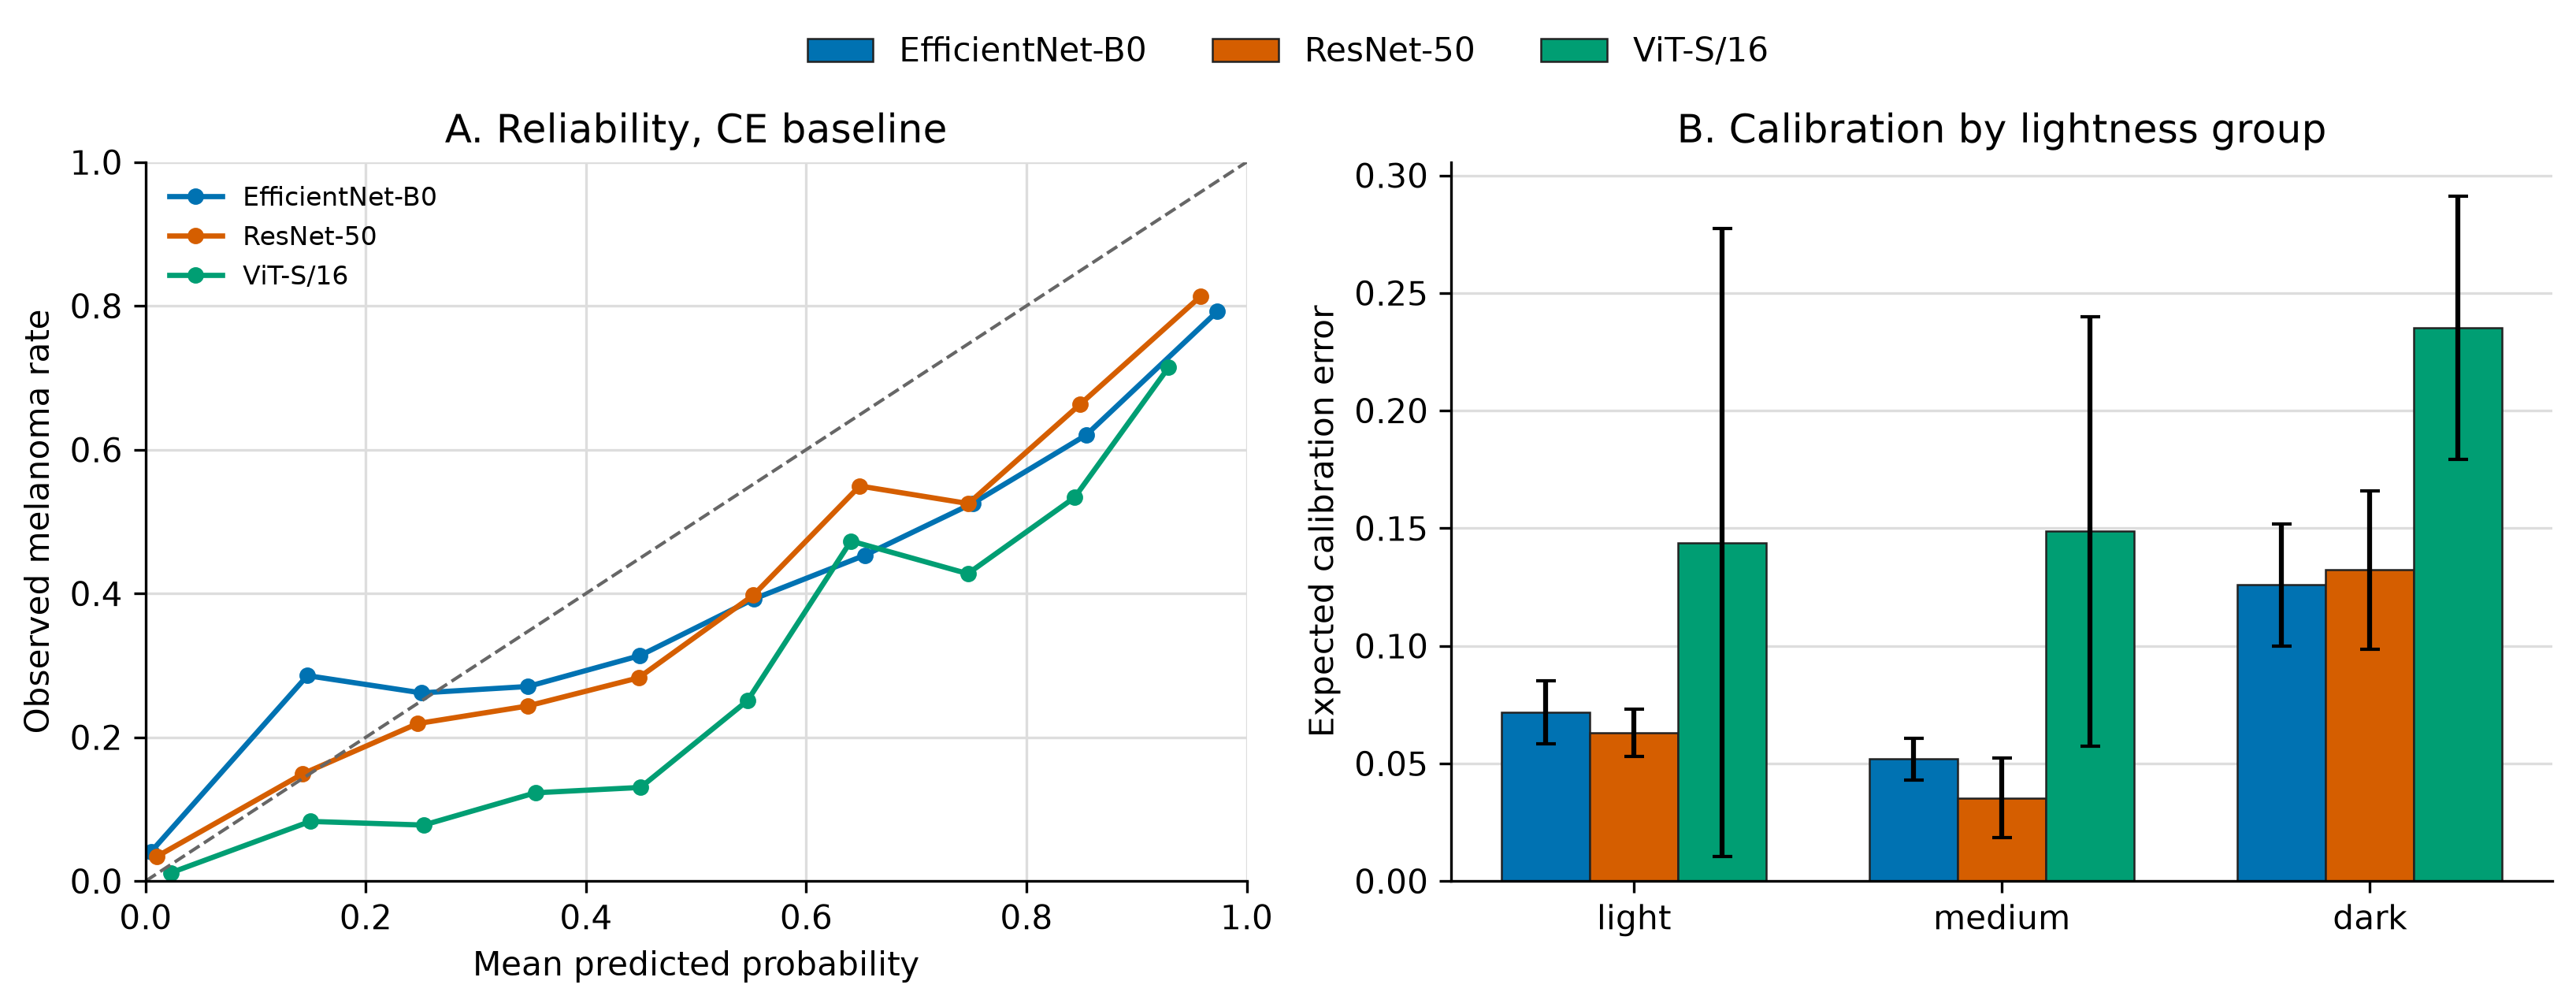
\includegraphics[width=\linewidth]{calibration_reliability.png}
  \caption{Calibration at the CE baseline. (A) Reliability curves for the three architectures. (B) Expected calibration error by lightness group, mean and seed standard deviation across the CE-baseline runs.}
  \label{fig:calibration}
\end{figure}

\subsection{Fairness across lightness strata}

The test set contains 644 light images with 81 melanomas, 840 medium images with 99 melanomas, and 43 dark images with 6 melanomas at the pre-declared cutoff $L^*\leq55$. The dark stratum is 2.8\% of the test set and 3.2\% of the melanoma cases.

Table~\ref{tab:fairness} reports the per-group sensitivity at 95\% specificity for the nine Stage 2 configurations at the pre-declared cutoff. At this cutoff the dark stratum has the lowest AUC in all nine configurations, 0.71 to 0.87, against 0.83 to 0.90 for light and 0.88 to 0.93 for medium. It also has the highest false positive rate, 0.08 to 0.19, against 0.04 to 0.07 for the other two groups.

The dark AUC differences are not statistically supported. Across the three cutoffs, none of the 54 dark-versus-light and dark-versus-medium AUC comparisons has a bootstrap interval that excludes zero. The dark AUC deficit is therefore a descriptive feature of the strict cutoff, not a confirmed group difference. The false positive rate is more consistent: it is 0.126 at $L^*\leq55$, 0.086 at $L^*\leq58$, and 0.073 at $L^*\leq60$, against 0.047 to 0.050 for light and medium at every cutoff. The intervals around these group rates remain wide.

Dark sensitivity is 0.500 with 6 melanomas, 0.648 with 12, and 0.580 with 23. It is not consistently lower than light sensitivity, and the intervals are wide.

The adjusted models in Table~\ref{tab:adjusted} separate false positives from false negatives. The most robust fairness result is the false-negative association: the $L^*$ odds ratio is 1.74 for ResNet-50, 1.66 for EfficientNet-B0, and 1.75 for ViT-S/16, and all three intervals exclude 1. Lighter skin is associated with more missed melanomas. The false-positive association points in the opposite direction, with $L^*$ odds ratios of 0.78, 0.88, and 0.77, but the interval excludes 1 only for ResNet-50. Lesion contrast is associated with more false positives for all three architectures (OR 2.05, 1.69, and 2.42) and with fewer false negatives for ViT-S/16 (OR 0.48; the other two intervals include 1).

The error-type pattern is therefore suggestive but not symmetric. The supported finding is the false-negative lightness association; the false-positive association and the contrast effects are directionally consistent but imprecise. A single sensitivity or AUC summary hides this distinction.

\begin{table}[t]
\centering
\small
\caption{Lightness-stratified test sensitivity at 95\% specificity. Values are mean and standard deviation across three seeds. The dark stratum contains 43 test images and six melanoma cases. These are image-based lightness groups, not clinical Fitzpatrick labels.}
\label{tab:fairness}
\resizebox{\textwidth}{!}{%
\begin{tabular}{lcccccc}
\toprule
Configuration & Light sens & Medium sens & Dark sens & Dark AUC & Dark FPR & Dark $n$ / pos. \\
\midrule
EfficientNet-B0 / CE & 0.477 $\pm$ 0.031 & 0.609 $\pm$ 0.050 & 0.722 $\pm$ 0.096 & 0.871 & 0.117 & 43 / 6 \\
EfficientNet-B0 / CE+strong & 0.519 $\pm$ 0.054 & 0.599 $\pm$ 0.086 & 0.556 $\pm$ 0.096 & 0.833 & 0.090 & 43 / 6 \\
EfficientNet-B0 / Focal+CB & 0.420 $\pm$ 0.064 & 0.522 $\pm$ 0.076 & 0.500 $\pm$ 0.167 & 0.806 & 0.081 & 43 / 6 \\
ResNet-50 / CE & 0.502 $\pm$ 0.036 & 0.633 $\pm$ 0.050 & 0.444 $\pm$ 0.096 & 0.803 & 0.117 & 43 / 6 \\
ResNet-50 / CE+strong & 0.527 $\pm$ 0.026 & 0.603 $\pm$ 0.038 & 0.556 $\pm$ 0.096 & 0.854 & 0.135 & 43 / 6 \\
ResNet-50 / Focal+CB & 0.399 $\pm$ 0.093 & 0.481 $\pm$ 0.066 & 0.722 $\pm$ 0.192 & 0.848 & 0.162 & 43 / 6 \\
ViT-S/16 / CE & 0.342 $\pm$ 0.091 & 0.451 $\pm$ 0.065 & 0.333 $\pm$ 0.167 & 0.740 & 0.144 & 43 / 6 \\
ViT-S/16 / CE+strong & 0.407 $\pm$ 0.054 & 0.471 $\pm$ 0.132 & 0.222 $\pm$ 0.096 & 0.763 & 0.126 & 43 / 6 \\
ViT-S/16 / Focal+CB & 0.362 $\pm$ 0.062 & 0.586 $\pm$ 0.010 & 0.389 $\pm$ 0.096 & 0.712 & 0.189 & 43 / 6 \\
\bottomrule
\end{tabular}
}
\end{table}

\begin{table}[t]
\centering
\small
\caption{Dark-skin threshold sensitivity at 95\% specificity. Values are means across the nine CE-baseline runs. The dark AUC gap is present at $L^*\leq55$ but not at $L^*\leq58$ or $60$, while the dark false positive rate remains elevated at every cutoff. These are image-based lightness groups, not clinical Fitzpatrick labels.}
\label{tab:darkskin}
\begin{tabular}{llccccc}
\toprule
$L^*$ cutoff & Group & $n$ & Melanomas & Sensitivity & AUC & FPR \\
\midrule
55 & light & 644 & 81 & 0.440 & 0.868 & 0.050 \\
 & medium & 840 & 99 & 0.565 & 0.911 & 0.049 \\
 & dark & 43 & 6 & 0.500 & 0.805 & 0.126 \\
\midrule
58 & light & 644 & 81 & 0.440 & 0.868 & 0.050 \\
 & medium & 777 & 93 & 0.550 & 0.908 & 0.048 \\
 & dark & 106 & 12 & 0.648 & 0.891 & 0.086 \\
\midrule
60 & light & 644 & 81 & 0.440 & 0.868 & 0.050 \\
 & medium & 704 & 82 & 0.556 & 0.912 & 0.047 \\
 & dark & 179 & 23 & 0.580 & 0.881 & 0.073 \\
\bottomrule
\end{tabular}
\end{table}

\begin{table}[t]
\centering
\small
\caption{Adjusted odds ratios for false positives and false negatives. Each model includes perilesional $L^*$, lesion contrast, log lesion area, age, sex, and anatomical site. Odds ratios are per one standard deviation; intervals are lesion-cluster bootstrap 95\% CIs. The pooled error model is not shown because the $L^*$ effects on false positives and false negatives have opposite signs.}
\label{tab:adjusted}
\resizebox{\textwidth}{!}{%
\begin{tabular}{llcc}
\toprule
Error type & Architecture & $L^*$ OR (95\% CI) & Contrast OR (95\% CI) \\
\midrule
False positive & ResNet-50 & 0.78 (0.61 to 0.94) & 2.05 (1.66 to 2.68) \\
 & EfficientNet-B0 & 0.88 (0.67 to 1.11) & 1.69 (1.39 to 2.14) \\
 & ViT-S/16 & 0.77 (0.57 to 1.03) & 2.42 (1.94 to 3.14) \\
\midrule
False negative & ResNet-50 & 1.74 (1.11 to 2.58) & 0.58 (0.35 to 1.02) \\
 & EfficientNet-B0 & 1.66 (1.16 to 2.34) & 0.74 (0.51 to 1.13) \\
 & ViT-S/16 & 1.75 (1.14 to 2.60) & 0.48 (0.29 to 0.75) \\
\bottomrule
\end{tabular}
}
\end{table}


\begin{figure}[t]
  \centering
  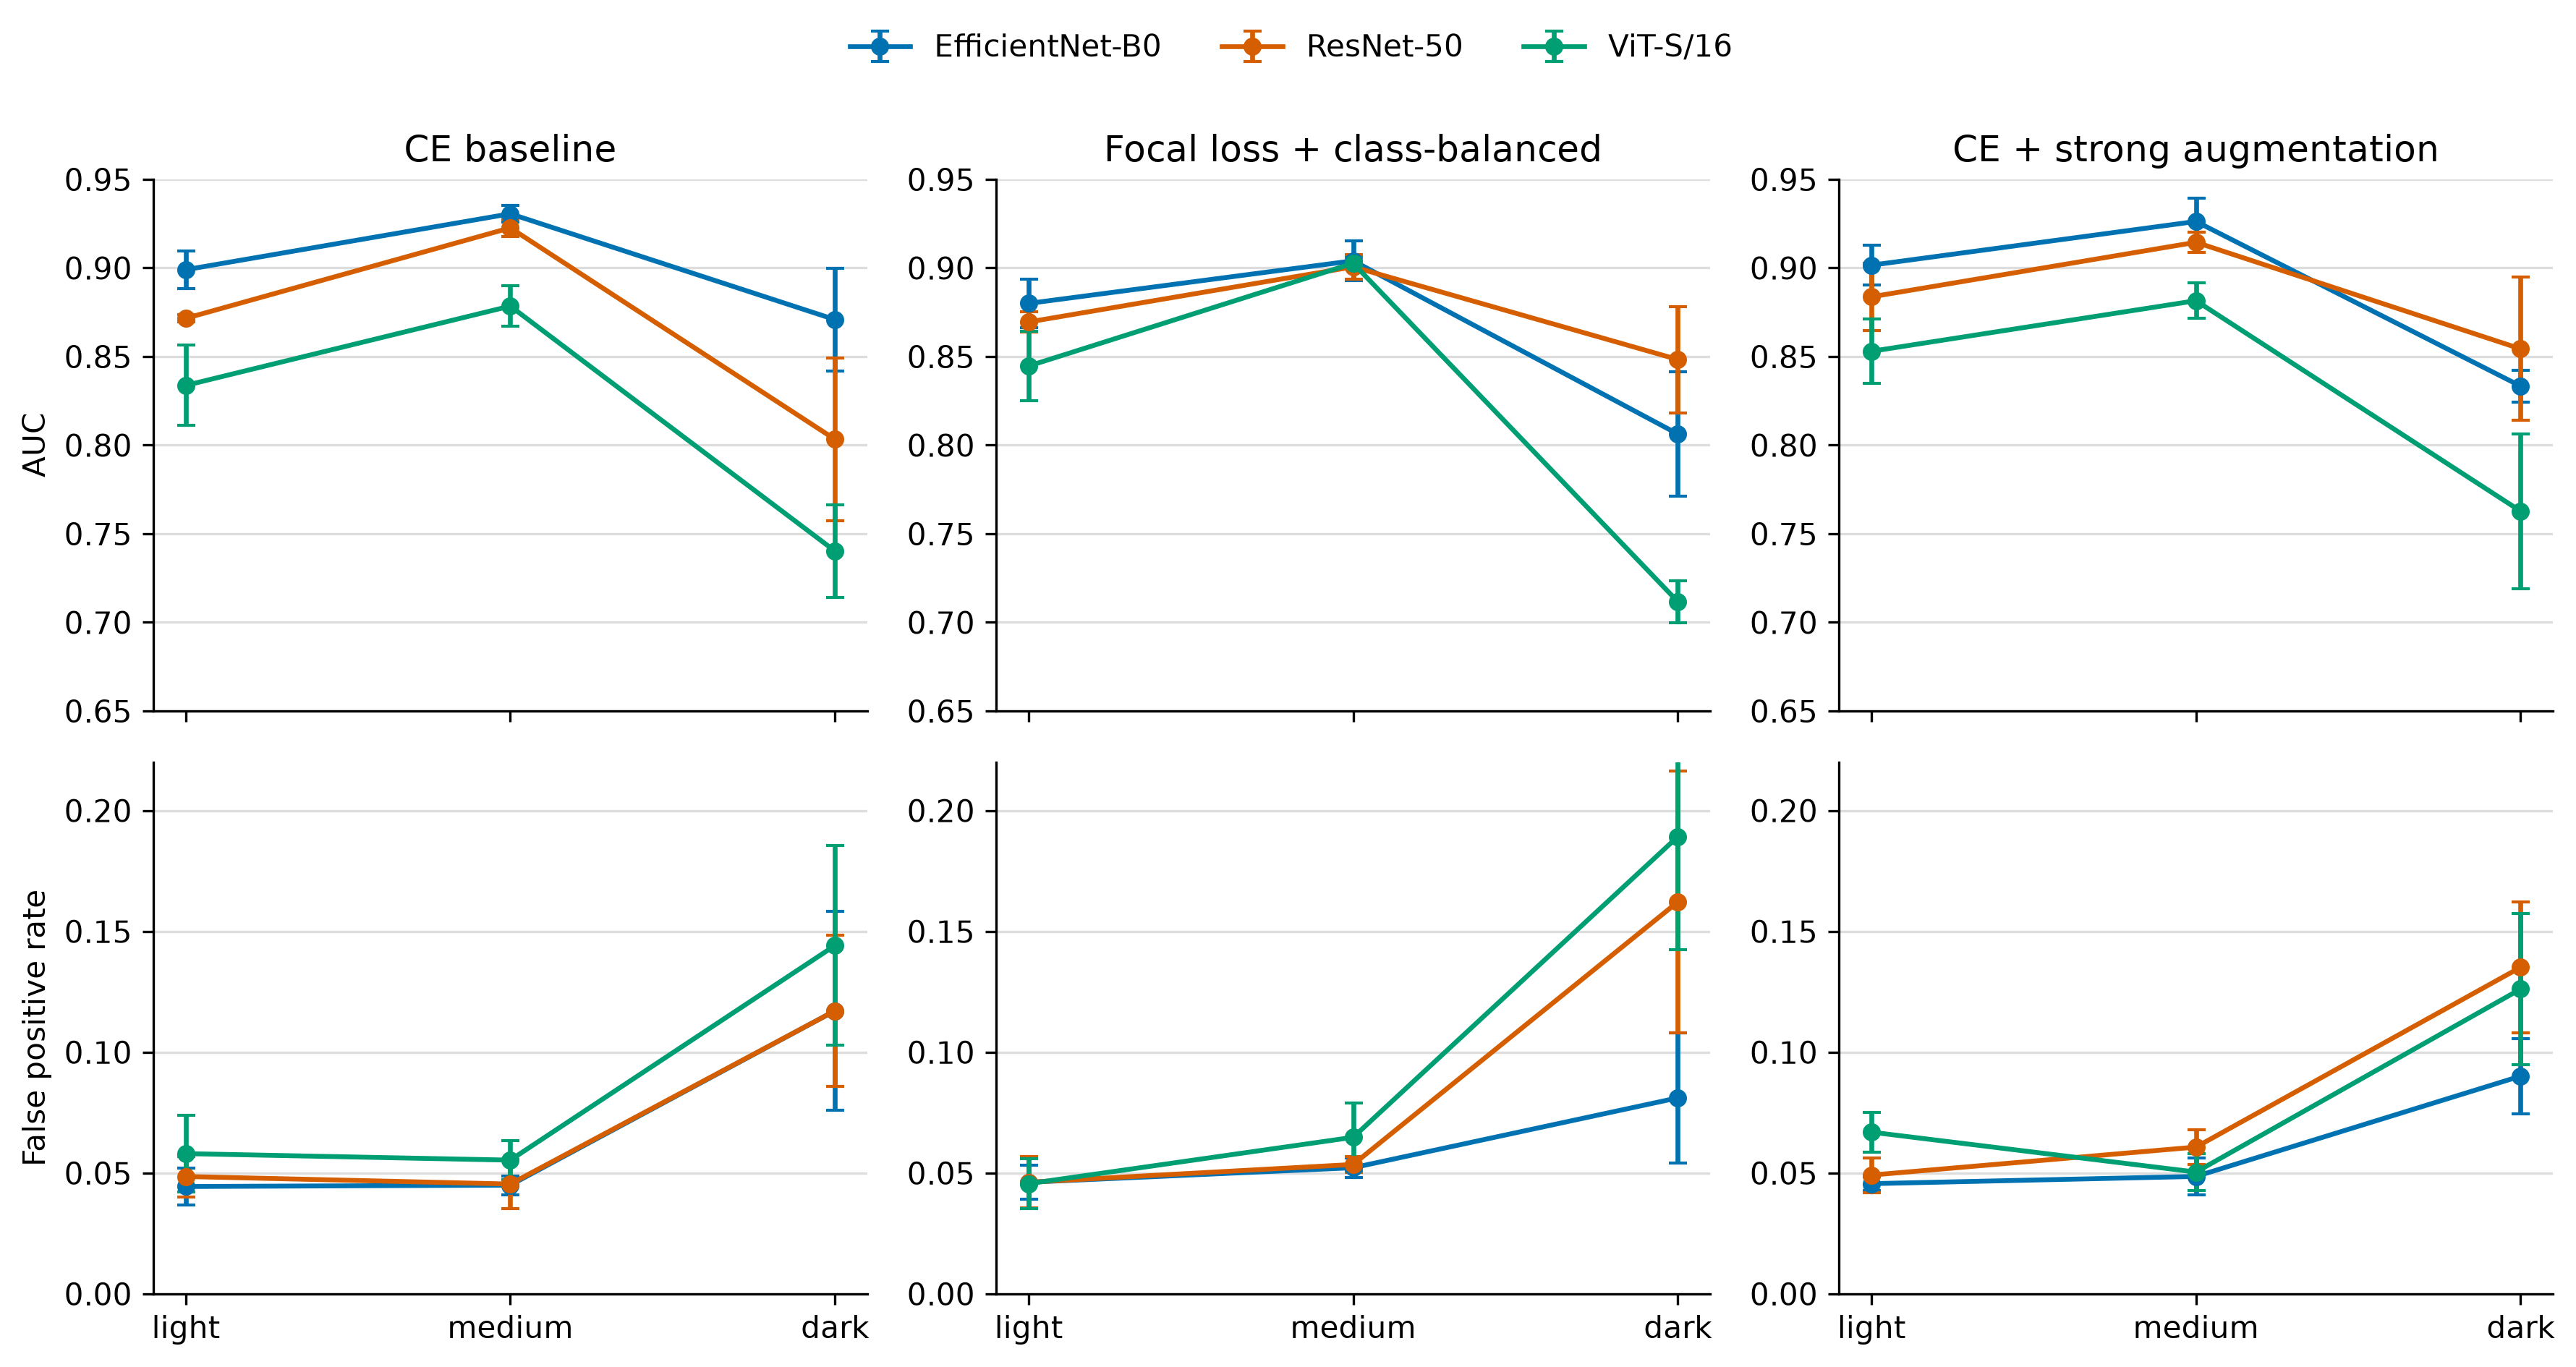
\includegraphics[width=\linewidth]{fairness_by_tone.png}
  \caption{AUC and false positive rate by lightness group for the nine Stage 2 configurations at the pre-declared cutoff $L^*\leq55$. Columns are training conditions and lines are architectures. Points are means across three seeds; error bars are seed standard deviations. The dark stratum contains 43 test images and six melanoma cases.}
  \label{fig:fairness}
\end{figure}

\begin{figure}[t]
  \centering
  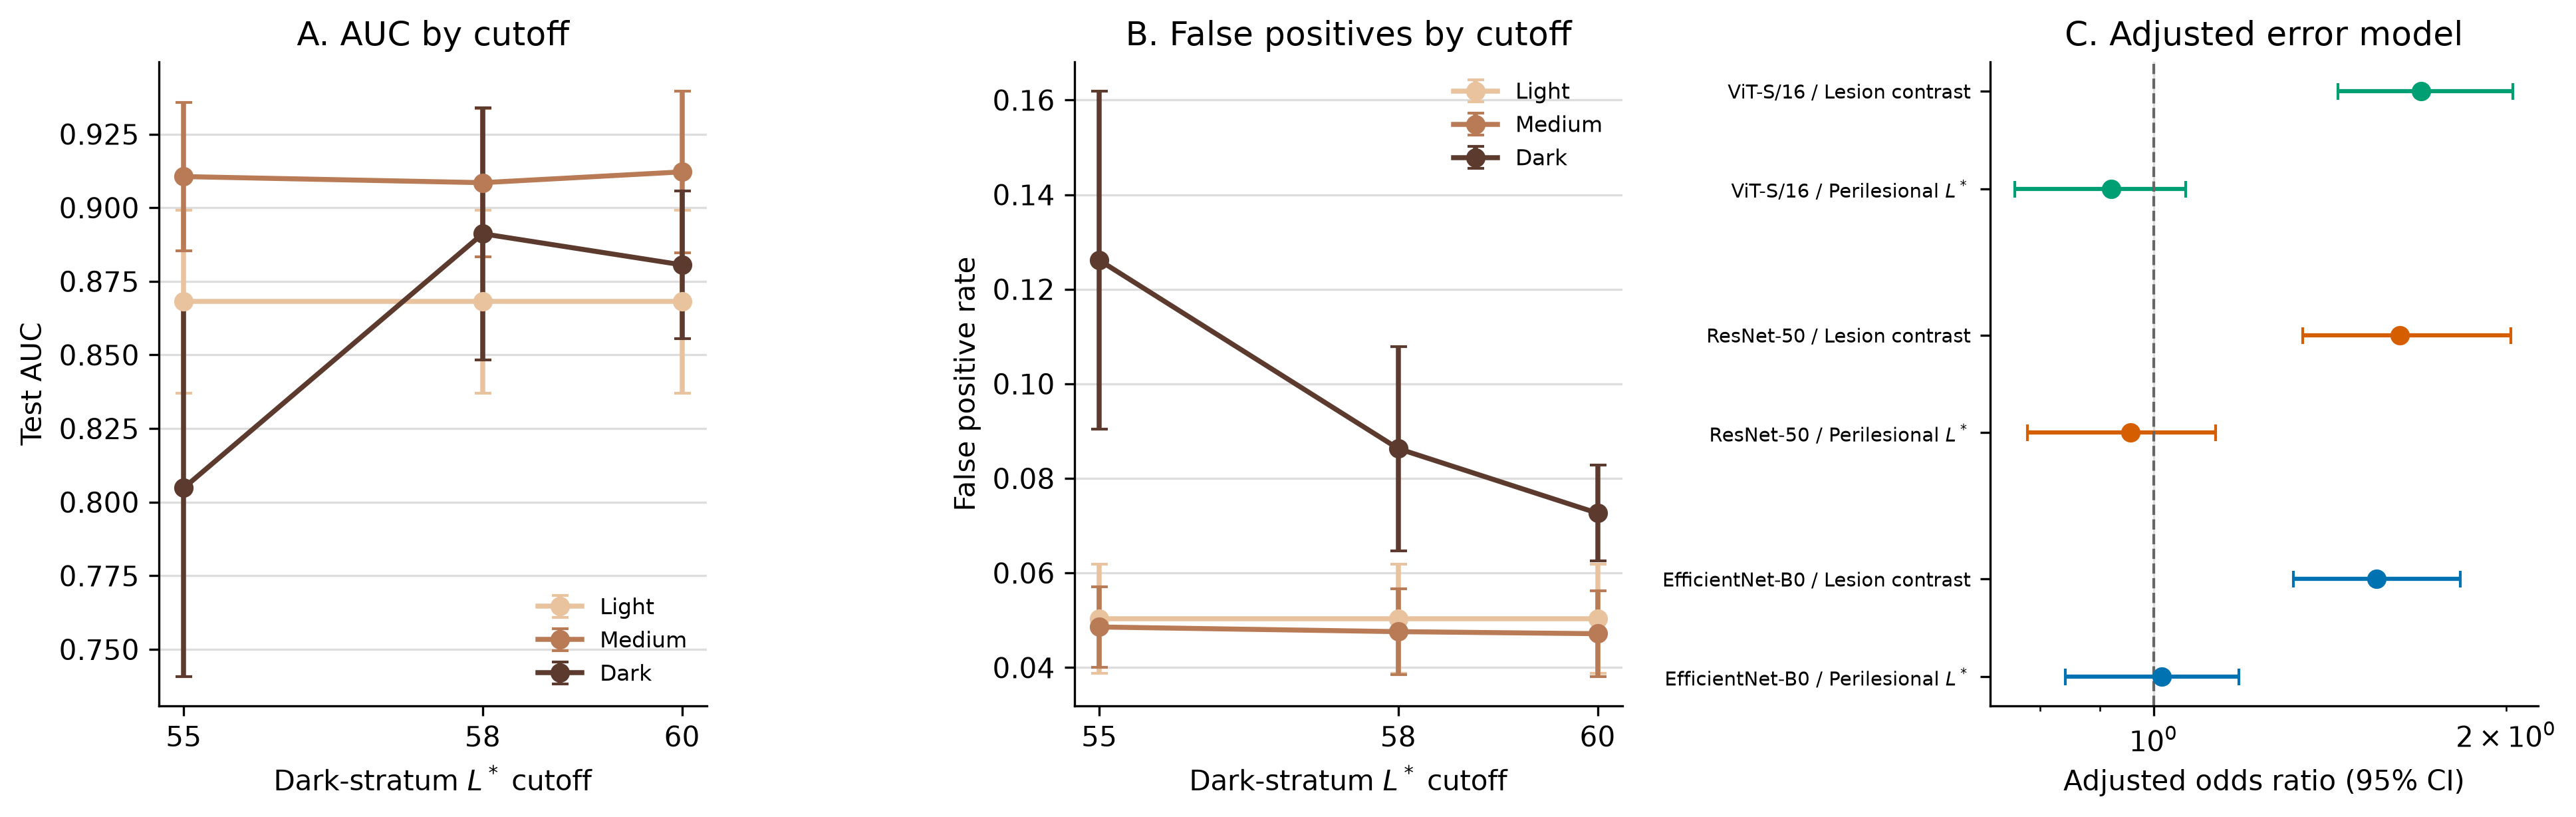
\includegraphics[width=\linewidth]{dark_skin_robustness.png}
  \caption{Dark-skin robustness. (A) AUC by $L^*$ cutoff. (B) False positive rate by cutoff. (C) Adjusted odds ratios for the pooled error model, per standard deviation, with lesion-cluster bootstrap 95\% CIs. The false-positive and false-negative models are reported separately in Table~\ref{tab:adjusted}.}
  \label{fig:darkskin}
\end{figure}

\subsection{Quantitative XAI}
\label{sec:xai}

Table~\ref{tab:xai} reports attribution mass inside the lesion, pointing-game accuracy, attribution IoU, and error rate for the CE-baseline models. Grad-CAM targets the true class, so a false-negative heatmap describes the evidence for melanoma rather than the benign prediction. Table~\ref{tab:xaicorr} reports the Spearman correlations. The sample contains 129 dark images and 18 melanomas across the three seeds, and 450 light and 450 medium images.

Attribution mass inside the lesion is highest in the light stratum for all three architectures. EfficientNet-B0 falls from $0.450$ to $0.368$ to $0.331$ across light, medium, and dark. ViT-S/16 falls from $0.341$ to $0.260$ and then stays near $0.261$. ResNet-50 falls from $0.571$ to $0.480$ and then to $0.465$. The mass-tone correlation is negative and significant for every architecture: $-0.176$ for EfficientNet-B0, $-0.174$ for ResNet-50, and $-0.181$ for ViT-S/16, all with $p<10^{-7}$.

Pointing-game accuracy is lowest in the dark stratum in every case: $0.448$ for EfficientNet-B0, $0.636$ for ResNet-50, and $0.248$ for ViT-S/16. Attribution IoU follows the same direction for EfficientNet-B0 and ViT-S/16, and is lower in the dark stratum than the medium stratum for ResNet-50 ($0.301$ vs $0.346$).

The mass-error correlation is architecture-dependent. It is negative for ResNet-50 ($-0.230$, $p<10^{-13}$) and EfficientNet-B0 ($-0.129$, $p<10^{-4}$), and positive for ViT-S/16 ($+0.136$, $p<10^{-4}$). Higher attribution mass inside the lesion is associated with fewer errors for the CNNs and with more errors for the ViT. The false-negative and false-positive mass values do not separate consistently: false negatives vs false positives are $0.374$ vs $0.260$ for EfficientNet-B0, $0.346$ vs $0.349$ for ResNet-50, and $0.420$ vs $0.344$ for ViT-S/16. The XAI signal is a group-level tone gradient, not a consistent per-image error marker.

Figure~\ref{fig:xai} shows the group pattern. ResNet-50 localizes best in absolute terms and has the highest dark-stratum attribution mass, but its dark false positive rate is not the lowest. Localization quality and error rate move together across tone groups, but they do not rank architectures the same way.

\begin{table}[t]
\centering
\small
\caption{Quantitative XAI at the CE baseline on the HAM10000 test split. Grad-CAM targets the true class. Each architecture uses three seeds and a tone-stratified sample of 343 test images per seed. Attribution mass is the fraction of the heatmap inside the lesion mask. Values are means across seeds.}
\label{tab:xai}
\resizebox{\textwidth}{!}{%
\begin{tabular}{llcccccc}
\toprule
Architecture & Tone group & $n$ & $n$ positive & Attribution mass & Pointing game & Attribution IoU & Error rate \\
\midrule
\multirow{3}{*}{ResNet-50} & light & 450 & 36 & 0.571 & 0.847 & 0.387 & 0.076 \\
 & medium & 450 & 54 & 0.480 & 0.777 & 0.346 & 0.078 \\
 & dark & 129 & 18 & 0.465 & 0.636 & 0.301 & 0.178 \\
\midrule
\multirow{3}{*}{EfficientNet-B0} & light & 450 & 36 & 0.450 & 0.702 & 0.324 & 0.076 \\
 & medium & 450 & 54 & 0.368 & 0.598 & 0.280 & 0.091 \\
 & dark & 129 & 18 & 0.331 & 0.448 & 0.195 & 0.140 \\
\midrule
\multirow{3}{*}{ViT-S/16} & light & 450 & 36 & 0.341 & 0.607 & 0.273 & 0.109 \\
 & medium & 450 & 54 & 0.260 & 0.391 & 0.185 & 0.116 \\
 & dark & 129 & 18 & 0.261 & 0.248 & 0.144 & 0.217 \\
\bottomrule
\end{tabular}
}
\end{table}

\begin{table}[t]
\centering
\small
\caption{Spearman correlations between attribution mass inside the lesion, lightness group, and error status at the CE baseline. Tone is coded light $=0$, medium $=1$, dark $=2$. A negative mass-tone correlation means less attribution inside the lesion on darker images.}
\label{tab:xaicorr}
\begin{tabular}{lccccc}
\toprule
Architecture & Images & $\rho$ (mass, tone) & $p$ & $\rho$ (mass, error) & $p$ \\
\midrule
EfficientNet-B0 & 1011 & -0.176 & $1.9\times10^{-8}$ & -0.129 & $4.2\times10^{-5}$ \\
ResNet-50 & 1028 & -0.174 & $2.0\times10^{-8}$ & -0.230 & $9.1\times10^{-14}$ \\
ViT-S/16 & 1029 & -0.181 & $5.1\times10^{-9}$ & 0.136 & $1.2\times10^{-5}$ \\
\bottomrule
\end{tabular}
\end{table}


\begin{figure}[t]
  \centering
  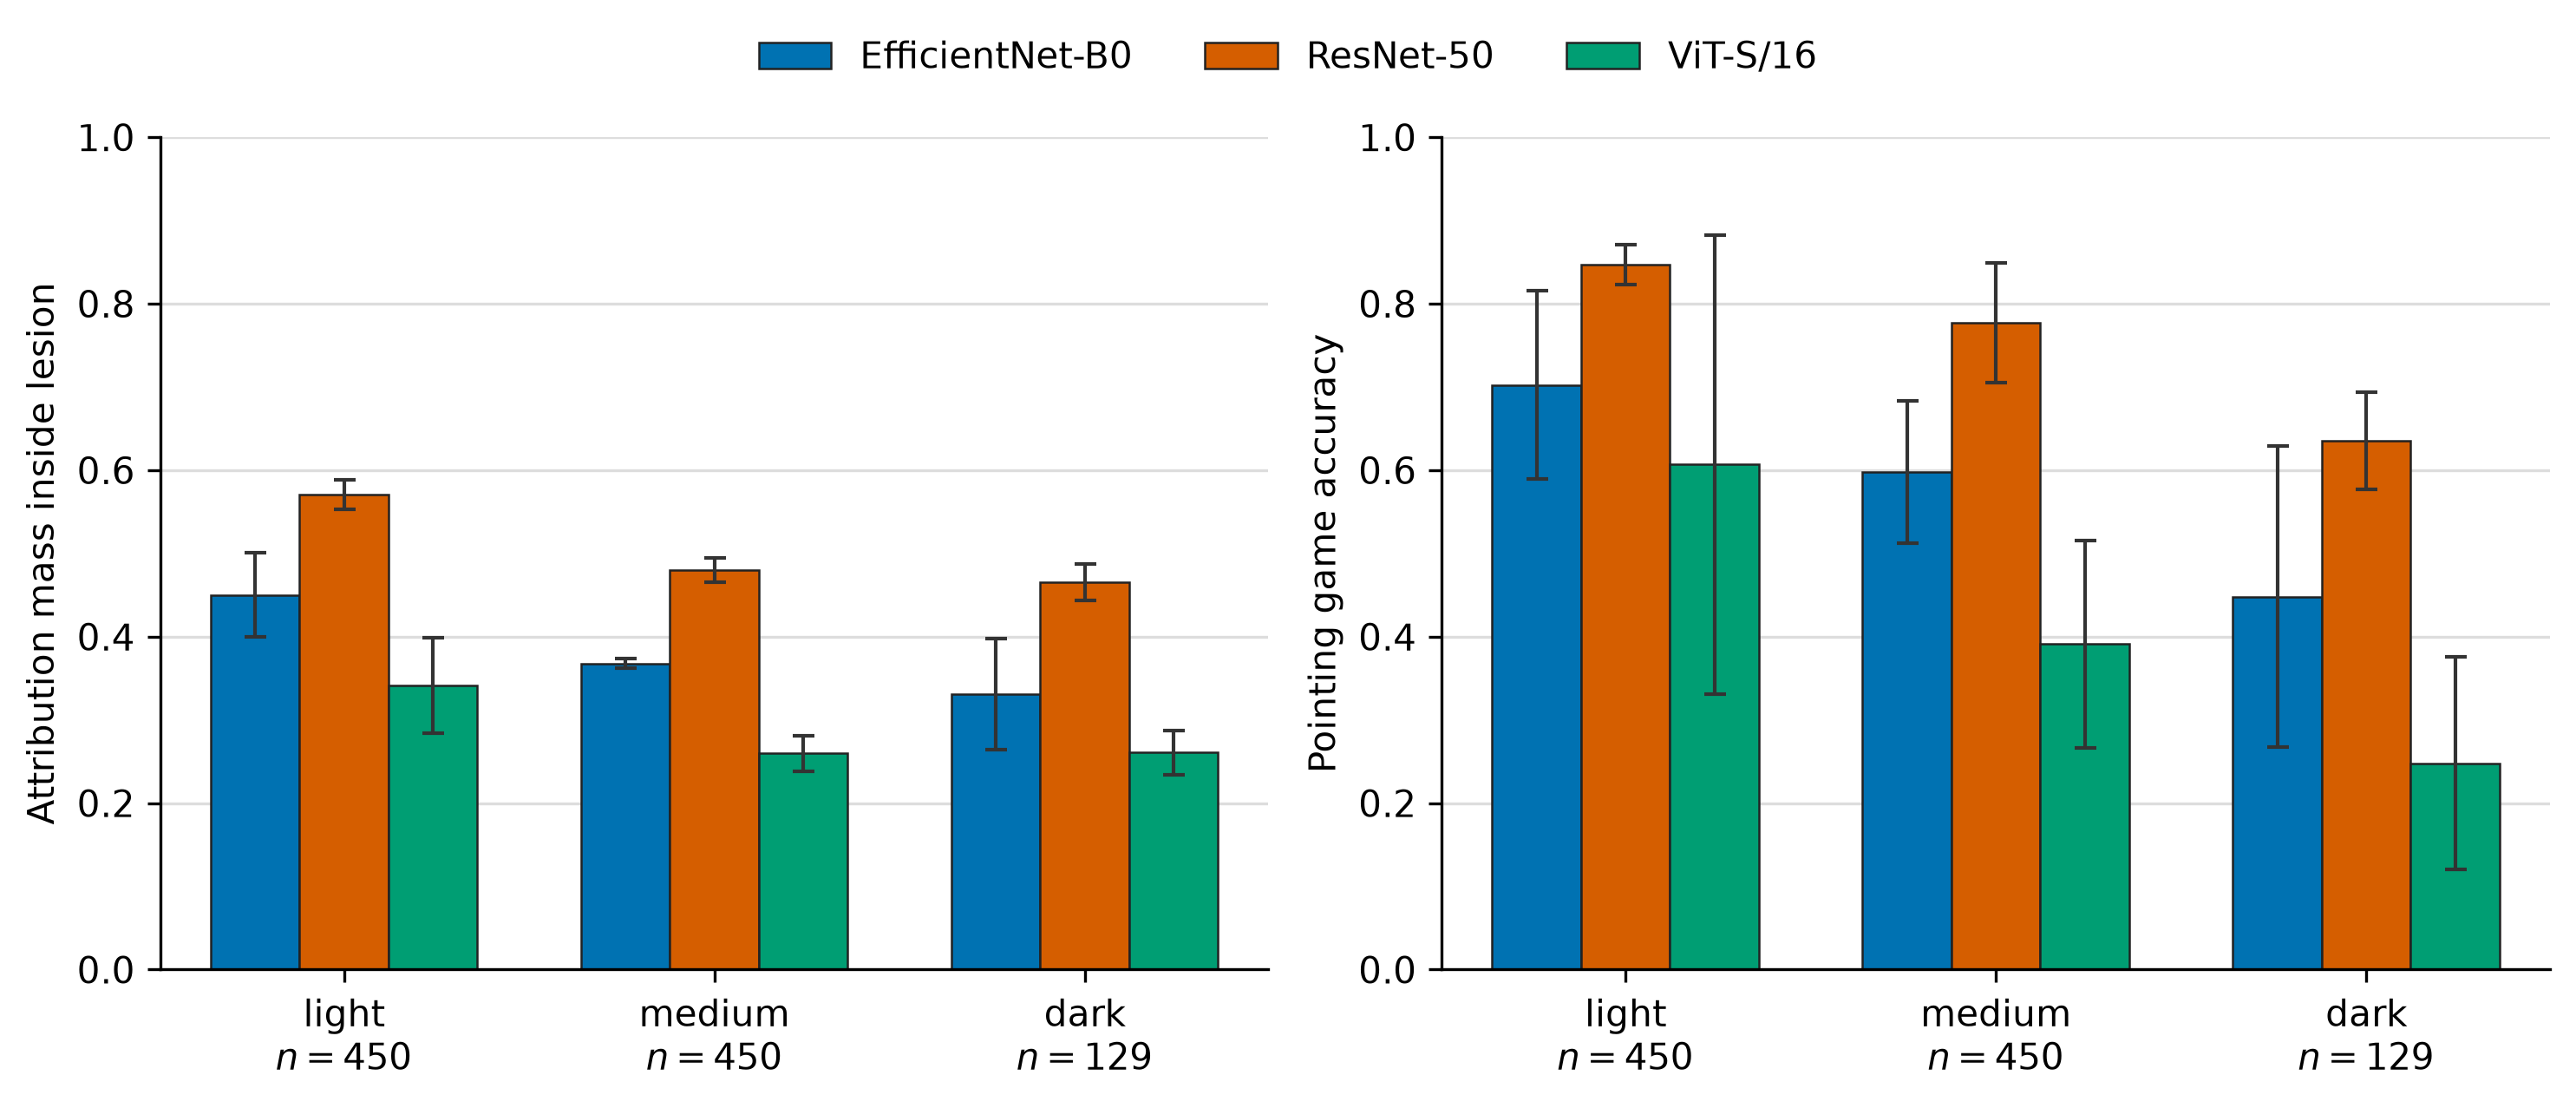
\includegraphics[width=\linewidth]{xai_by_tone.png}
  \caption{Attribution mass inside the lesion and pointing-game accuracy by lightness group for the three CE-baseline architectures. Grad-CAM targets the true class. Bars are means across three seeds; error bars are seed standard deviations. The sample contains all 43 dark test images per seed and 150 randomly drawn light and medium images per seed.}
  \label{fig:xai}
\end{figure}

\subsection{External tone-labeled validation}
\label{sec:external}

Table~\ref{tab:external} reports the HIBA dermoscopic subset for the CE-baseline models: 1,280 images and 196 melanomas. We applied the HAM10000 validation threshold at 95\% specificity without refitting. HIBA contains Fitzpatrick I-IV only, and 108 images have no Fitzpatrick label.

Sensitivity drops on the external set. ResNet-50 reaches $0.391\pm0.056$ at $0.944$ specificity, EfficientNet-B0 reaches $0.396\pm0.036$ at $0.922$, and ViT-S/16 reaches $0.221\pm0.130$ at $0.967$. The AUCs are $0.807\pm0.018$, $0.782\pm0.024$, and $0.791\pm0.027$. On the HAM10000 test set the same models reached $0.57$, $0.56$, and $0.40$ sensitivity at 95\% specificity. Both CNNs outperform the transformer on external sensitivity, but the two CNNs are within half a point of each other. The absolute drop is consistent with domain shift between the Argentine HIBA collection and HAM10000.

The per-type estimates do not show a monotonic skin-tone gradient. For Fitzpatrick I, II, and III, CNN sensitivity ranges from $0.35$ to $0.43$, and the ViT is lower at $0.20$ to $0.33$. Fitzpatrick IV contains 25 images and no melanomas, so sensitivity is undefined and only specificity can be estimated. The group sizes are unbalanced: 804 of the 1,280 images are type II. HIBA cannot test the dark-skin claim, because it has almost no type IV melanoma cases and no type V-VI images at all.

Table~\ref{tab:externalcond} compares all three conditions on HIBA. The focal condition raises ViT-S/16 sensitivity from $0.221$ to $0.315$, lowers ResNet-50 from $0.391$ to $0.315$, and lowers EfficientNet-B0 from $0.396$ to $0.253$. The ViT change is $+0.219$, $+0.127$, and $-0.067$ across seeds, with a mean of $+0.094$; the CNN changes are negative in every seed for EfficientNet-B0 and in two of three seeds for ResNet-50. The focal evidence is therefore directionally consistent for the CNNs and suggestive but not confirmatory for the ViT.

Strong augmentation is the best external condition for all three architectures. It raises sensitivity from $0.391$ to $0.480$ for ResNet-50, from $0.396$ to $0.406$ for EfficientNet-B0, and from $0.221$ to $0.391$ for ViT-S/16. The corresponding AUCs are $0.835$, $0.847$, and $0.824$, and the oracle 95\% specificity sensitivities are $0.408$, $0.427$, and $0.389$. The near-neutral in-domain effect of strong augmentation therefore does not transfer: the condition designed to simulate domain shift improves external generalization. This is a more favorable external result for the Stage 1 winner than the in-domain benchmark suggested.

At the oracle 95\% specificity threshold, focal loss leaves the CNN sensitivity below the CE baseline and raises the ViT, while strong augmentation raises all three above the CE baseline. The external AUC ordering also differs from the in-domain ordering. Under focal loss the external AUC ranking is ViT-S/16 $0.794$, ResNet-50 $0.774$, and EfficientNet-B0 $0.722$, while the in-domain focal ranking is EfficientNet-B0 $0.891$, ResNet-50 $0.884$, and ViT-S/16 $0.872$. HIBA is a different imaging regime, not a clean replication.

The external validation supports a limited conclusion. Strong augmentation generalizes best, the CNN sensitivity loss under focal loss is consistent in direction, and the ViT focal gain is possible but seed-dependent. The absolute performance of the CE baseline does not transfer, so the operating point needs recalibration for a new source. The tone-specific claim remains limited to the image-based lightness strata in HAM10000 and to the error-type associations reported above.

\begin{table}[t]
\centering
\small
\caption{External validation on the HIBA dermoscopic subset for the CE-baseline models (1,280 images, 196 melanomas). The threshold is the HAM10000 validation threshold at 95\% specificity, frozen before the external evaluation. Values are mean and standard deviation across three seeds. Fitzpatrick IV contains 25 images and no melanomas, so sensitivity is undefined. The 108 images without a Fitzpatrick label are included in the All row only.}
\label{tab:external}
\resizebox{\textwidth}{!}{%
\begin{tabular}{llcccccc}
\toprule
Architecture & Fitzpatrick & $n$ & Melanomas & Sensitivity & Specificity & AUC \\
\midrule
\multirow{5}{*}{ResNet-50} & I & 97 & 25 & 0.360 $\pm$ 0.069 & 0.954 $\pm$ 0.021 & 0.679 $\pm$ 0.031 \\
 & II & 804 & 144 & 0.403 $\pm$ 0.066 & 0.922 $\pm$ 0.011 & 0.780 $\pm$ 0.020 \\
 & III & 246 & 17 & 0.412 $\pm$ 0.000 & 0.978 $\pm$ 0.004 & 0.946 $\pm$ 0.011 \\
 & IV & 25 & 0 & -- & 1.000 $\pm$ 0.000 & -- \\
 & All & 1280 & 196 & 0.391 $\pm$ 0.056 & 0.944 $\pm$ 0.006 & 0.807 $\pm$ 0.018 \\
\midrule
\multirow{5}{*}{EfficientNet-B0} & I & 97 & 25 & 0.427 $\pm$ 0.061 & 0.940 $\pm$ 0.021 & 0.741 $\pm$ 0.068 \\
 & II & 804 & 144 & 0.389 $\pm$ 0.039 & 0.890 $\pm$ 0.010 & 0.745 $\pm$ 0.028 \\
 & III & 246 & 17 & 0.353 $\pm$ 0.059 & 0.974 $\pm$ 0.004 & 0.860 $\pm$ 0.044 \\
 & IV & 25 & 0 & -- & 0.987 $\pm$ 0.023 & -- \\
 & All & 1280 & 196 & 0.396 $\pm$ 0.036 & 0.922 $\pm$ 0.008 & 0.782 $\pm$ 0.024 \\
\midrule
\multirow{5}{*}{ViT-S/16} & I & 97 & 25 & 0.200 $\pm$ 0.144 & 0.995 $\pm$ 0.008 & 0.773 $\pm$ 0.061 \\
 & II & 804 & 144 & 0.227 $\pm$ 0.131 & 0.950 $\pm$ 0.033 & 0.777 $\pm$ 0.018 \\
 & III & 246 & 17 & 0.333 $\pm$ 0.189 & 0.994 $\pm$ 0.007 & 0.849 $\pm$ 0.053 \\
 & IV & 25 & 0 & -- & 1.000 $\pm$ 0.000 & -- \\
 & All & 1280 & 196 & 0.221 $\pm$ 0.129 & 0.967 $\pm$ 0.022 & 0.791 $\pm$ 0.027 \\
\bottomrule
\end{tabular}
}
\end{table}

\begin{table}[t]
\centering
\small
\caption{External validation on HIBA for all three training conditions. Thresholds are the frozen HAM10000 validation thresholds. Sensitivity at 95\% specificity uses an oracle threshold fitted on HIBA and is an upper bound, not a deployable result. Values are mean and standard deviation across three seeds.}
\label{tab:externalcond}
\resizebox{\textwidth}{!}{%
\begin{tabular}{llcccc}
\toprule
Architecture & Condition & Sensitivity & Specificity & AUC & Sens. at 95\% spec. \\
\midrule
ResNet-50 & CE & 0.391 $\pm$ 0.056 & 0.944 $\pm$ 0.006 & 0.807 $\pm$ 0.018 & 0.366 $\pm$ 0.036 \\
ResNet-50 & CE+strong & 0.480 $\pm$ 0.032 & 0.935 $\pm$ 0.011 & 0.835 $\pm$ 0.010 & 0.408 $\pm$ 0.044 \\
ResNet-50 & Focal+CB & 0.315 $\pm$ 0.070 & 0.925 $\pm$ 0.005 & 0.774 $\pm$ 0.017 & 0.245 $\pm$ 0.057 \\
EfficientNet-B0 & CE & 0.396 $\pm$ 0.036 & 0.922 $\pm$ 0.008 & 0.782 $\pm$ 0.024 & 0.311 $\pm$ 0.035 \\
EfficientNet-B0 & CE+strong & 0.406 $\pm$ 0.069 & 0.955 $\pm$ 0.014 & 0.847 $\pm$ 0.003 & 0.427 $\pm$ 0.024 \\
EfficientNet-B0 & Focal+CB & 0.253 $\pm$ 0.071 & 0.945 $\pm$ 0.018 & 0.722 $\pm$ 0.045 & 0.240 $\pm$ 0.040 \\
ViT-S/16 & CE & 0.221 $\pm$ 0.129 & 0.967 $\pm$ 0.022 & 0.791 $\pm$ 0.027 & 0.310 $\pm$ 0.084 \\
ViT-S/16 & CE+strong & 0.391 $\pm$ 0.108 & 0.940 $\pm$ 0.023 & 0.824 $\pm$ 0.018 & 0.389 $\pm$ 0.023 \\
ViT-S/16 & Focal+CB & 0.315 $\pm$ 0.052 & 0.954 $\pm$ 0.011 & 0.794 $\pm$ 0.011 & 0.335 $\pm$ 0.016 \\
\bottomrule
\end{tabular}
}
\end{table}

